% !TEX root = ../main.tex
\chapter{Les services web: Vue d'ensemble}
Ce chapitre établit une étude du fondement théorique de notre travail
à savoir les concepts de base du paradigme service Web.  Nous
commençons d'abord par présenter un tour d'horizon définissant
l'architecture de référence de ce paradigme ainsi que quelque
définitions proposées dans la littérature. Ensuite nous nous
intéressons à montrer les limitations de l'approche syntaxique de la
description de services web et l'apport de l'enrichissement sémantique
de cette dernière aux processus de la découverte et la composition de
services Web.

\newpage
\section{Définitions et caractéristiques}
\label{sec:ws-notions-de-base}

Les services Web est l'approche la plus populaire pour mettre en œuvre
une architecture SOA . Le terme service Web qualifie tout service
disponible par Internet, qui utilise un format standard (généralement
\acrshort{xml} ou \acrshort{json}) d'échange de messages, et qui n'est
pas lié à un système d'exploitation ou un langage de programmation
particulier.

\label{sec:ws-definition}
Curbera et al. \cite{curbera2001web} a définissent un service web
comme \emph{``une application réseau capable d'interagir par le moyen
  des standards et des protocoles via des interfaces bien spécifiés,
  dans lequel est décris utilisant un langage de description
  fonctionnel standardisé''}.

Les services Web ont été proposés initialement par IBM
\cite{kreger2001web} et Microsoft, puis en standardisés par le
\acrshort{w3c} \footnote{\url{http://www.w3.org/}} et définis
\cite{WSA} par :

\emph{``Un service web est un système conçu pour permettre
  d'interopérabilité des applications à travers un réseau.  Il est
  caractérisé par un format de description
  interprétable/compréhensible automatiquement par la machine,
  D'autres systèmes peuvent interagir avec le Service Web selon la
  manière prescrite dans sa description et en utilisant des messages
  SOAP, généralement transmis via le protocole HTTP et sérialisés en
  XML et en d'autres standards du Web ''}.

Cette définition surligne les caractéristiques clés de services Web
\cite{fremantle2002enterprise}:

\renewcommand{\descriptionlabel}[1]{\hspace{1cm}\textbullet~\textsf{#1}}
\begin{description}
\item[Basés sur des protocoles Internet] : L'utilisation de
  \acrshort{http} pour le transport des informations permet de
  traverser les contrôles d'accès dans un environnement hétérogène.

\item[Interopérables] : Le standard \textsc{SOAP} \cite{box2000simple}
  définit comme étant un protocole destiné à l'échange de messages
  structurés véhiculé généralement sur \textsc{HTTP} et sérialisé en
  \textsc{XML}, permettant le support pour l'interopérabilité.

\item[Basés sur XML] : Le méta-langage de balisage \textsc{XML}
  \textit{eXtensible Markup Language} est un standard Web ouvert par
  \textsc{W3C} \cite{bray1998extensible} offre un cadre standard pour
  la définition de documents Interprétable par des machines.
\end{description}

M. P. Papazoglou \cite{papazoglou2003service} de apporte une
autre définition de services web:\\ \emph{``Les services Web sont
des éléments auto-descriptifs et indépendants des plateformes
permettent la composition faible coût d’applications
distribuées. Les services Web effectuent des fonctions allant de
simples requêtes des processus métiers complexes. Les services Web
permettent aux organisations d’exposer leurs programmes résultats
sur Internet (ou sur un intranet) en utilisant des langages (basés
sur XML) et des protocoles standardisés et de les mettre en œuvre
via une interface auto-descriptive basée sur des formats
standardisés et ouverts''}

% TODO: make a comment on this def and introduce the web services %
% composition idea:

% \subsection{L'évolution des styles de services web}
% \label{sec:levol-des-styl}
% \input{content/evolution.tex}
% \newpage

\section{L'architecture de référence et technlogies associées}
\label{sec:reference-arch}
Cette architecture a été proposée afin de promouvoir
l'interopérabilité et l'extensibilité de services Web dans
l'ensemble, une architecture de base de services Web est constitué
d'un fournisseur du servicee \textit{(Provider)}, un annuaire des
services \textit{(Service Registry)}, et un client du service
\textit{(Service Requester)}. La figure \ref{fig:ws_roles} montre
comment ces trois rôles interagissent.

%!TEX root = ../main.tex

\begin{figure}[h]
    \centering 
    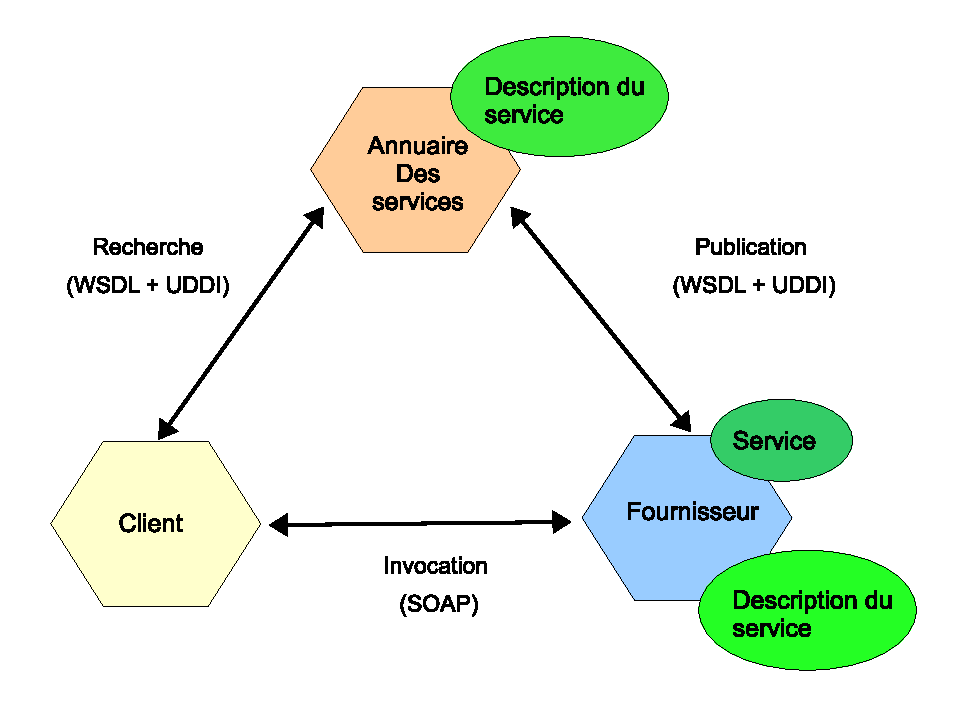
\includegraphics[width=1.1\textwidth]{figs/ws_roles.eps}
    \caption{Architecture de référence des services Web \cite{gottschalk2002introduction}}
    \label{fig:ws_roles}
\end{figure}
%%% Local Variables:
%%% mode: latex
%%% TeX-master: "../main.tex"
%%% End:

\renewcommand{\descriptionlabel}[1]{\hspace{1cm}\textbullet~\textsf{#1}}
\begin{description}
\item[Le fournisseur]: Un prestataire de services fournit l'interface
  pour le service Web et l'implémentation de l'application.

\item[L'annuaire]: Un registre de service est une façon dont les
  services Web sont officiellement publiés. Le registre de service est
  basée sur la spécification \textsc{UDDI} et reflète des informations
  sur les services fournis par le fournisseur de services.

\item[Le client]: Un client d'un service est le consommateur d'un
  service Web, il utilise le registre de service pour obtenir des
  informations et pour pouvoir accèder à un service Web.
\end{description}

Pour qu'une application profite de services Web, trois comportements
doivent avoir lieu : \textit{la publication} des descriptions du
service, \textit{la découverte} de ces descriptions et enfin
\textit{l'invocation} de services.

\renewcommand{\descriptionlabel}[1]{\hspace{1cm}\textbullet~\textsf{#1}}
\begin{description}
\item[Publier]: Pour être accessible, une description de service doit
  être publiée afin que le client puisse la trouver.

\item[Découvrir]: Lors de la découverte d'un service , le client
  interroge un annuaire (ou un registre) de services pour une
  catégorie requise de services et récupère une description
  détaillée.

\item[Invoquer (bind)]: le client peut ainsi invoquer une
  fonctionalité particulière dans le service cible utilisant les
  détails de liaison dans la description du service pour le localiser,
  contacter et l'appeler.
\end{description}

Les services Web sont construits autour de standards qui sont
\acrshort{soap}, \acrshort{wsdl} et \acrshort{uddi} assurant
respectivement leur communication, leur description et leur
découverte.

  \subsection{Communication: SOAP}
  \label{sec:soap}
  Développé par IBM\footnote{\url{http://www.ibm.com}} et
  Microsoft\footnote{\url{http://www.microsoft.com}}
  \cite{box2000simple}, Le langage \textsc{SOAP} est une
  recommandation \textsc{W3C} \cite{mitra2003soap} qui le définit
  comme étant un protocole destiné à l'échange de messages structurés,
  permettant d'invoquer des applications sur des réseaux distribués.

  \textsc{SOAP} est basé sur \textsc{XML} pour mettre en place un
  mécanisme valable d'échange des données indépendant du modèle de
  programmation de l'application et du système d'exploitation.

  Un message \textsc{SOAP} est un document XML constitué d'une
  enveloppe \textsc{SOAP} obligatoire, d'un en-tête \textsc{SOAP}
  facultatif et d'un corps \textsc{SOAP} obligatoire (voir la figure
  \ref{fig:soap-message-structure}):

  \begin{figure}[htbp]
    \centering
    \begin{subfigure}[b]{1\textwidth}        
	\centering
	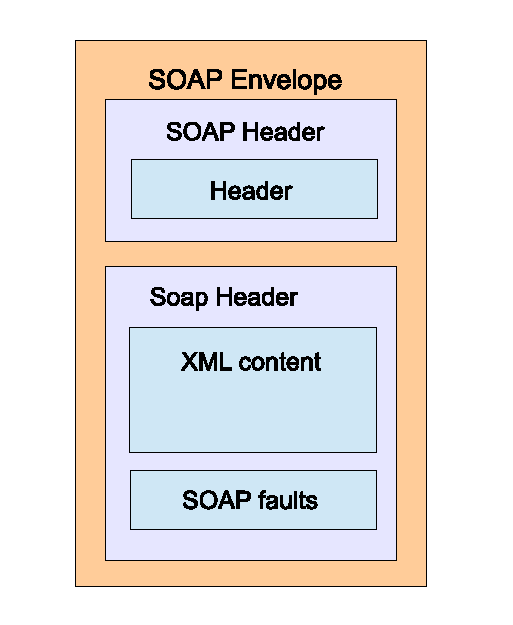
\includegraphics[width=0.5\textwidth]{figs/soap_structure.eps}
	\caption{ Les éléments d'un message \textsc{SOAP}}
	\label{fig:soap_structure}
    \end{subfigure}    

    \begin{subfigure}[b]{1\textwidth}
	\centering
	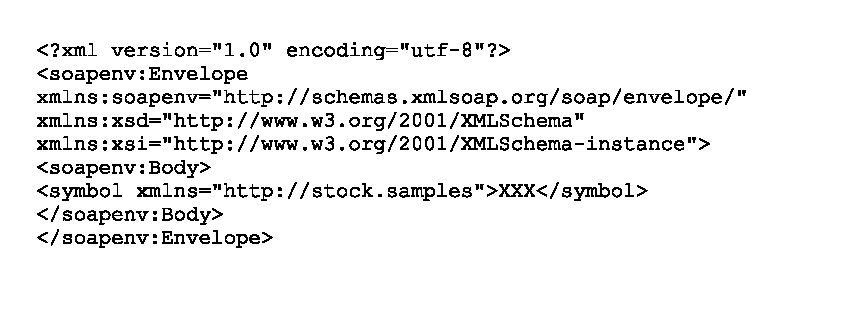
\includegraphics[width=1\textwidth]{figs/soap_message.eps}
	\caption{Exemple de message SOAP}
	\label{fig:soap-message}

    \end{subfigure}
    \caption{La structure d'un message \textsc{SOAP}}
    \label{fig:soap_all}
\end{figure}


  \renewcommand{\descriptionlabel}[1]{\hspace{1cm}\textbullet~\textsf{#1}}
  \begin{description}
  \item[Enveloppe \texttt{<Envelope>}]: L'élément racine du message
    \textsc{SOAP}, définissant le contexte du message, son
    destinataire et son contenu, il englobe l'en-tête et le corps.

  \item[En-tête \texttt{<Header>}]: Un mécanisme générique permettant
    d'ajouter des fonctions à un message \textsc{SOAP} d'une manière
    modulaire sans accord préalable entre les parties en
    communication.  Des exemples d'extension qui peuvent être
    implémentées comme des en-têtes sont des authentifications, des
    transactions, des paiements.
\newpage
  \item[Corps \texttt{<Body>}]: Contient les informations obligatoires
    destinées à l'ultime destinataire du message, il sert comme un
    container pour les informations mandataires à l'intention du
    récepteur du message. \textsc{SOAP} définit un élément pour le
    corps, qui est l'élément \texttt{<Fault>} (Erreur) utilisé pour
    rapporter les erreurs.
  \end{description}

  \subsection{Description: WSDL}
  \label{sec:wsdl}
  Le langage de description de services Web \acrshort{wsdl}
  \cite{christensen2001web, chinnici2007web} est une recommandation du
  \acrshort{w3c}, maintenant dans sa deuxième version.  \textsc{WSDL}
  est basé sur \textsc{XML} pour décrire les fonctions opérationnelles
  de services Web. La description \textsc{WSDL} est composée d'un
  interface et des implémentations. L'interface est une définition
  abstraite et réutilisable service qui peut être référencée par
  plusieurs implémentations.

  \begin{figure}[h]
    \centering
    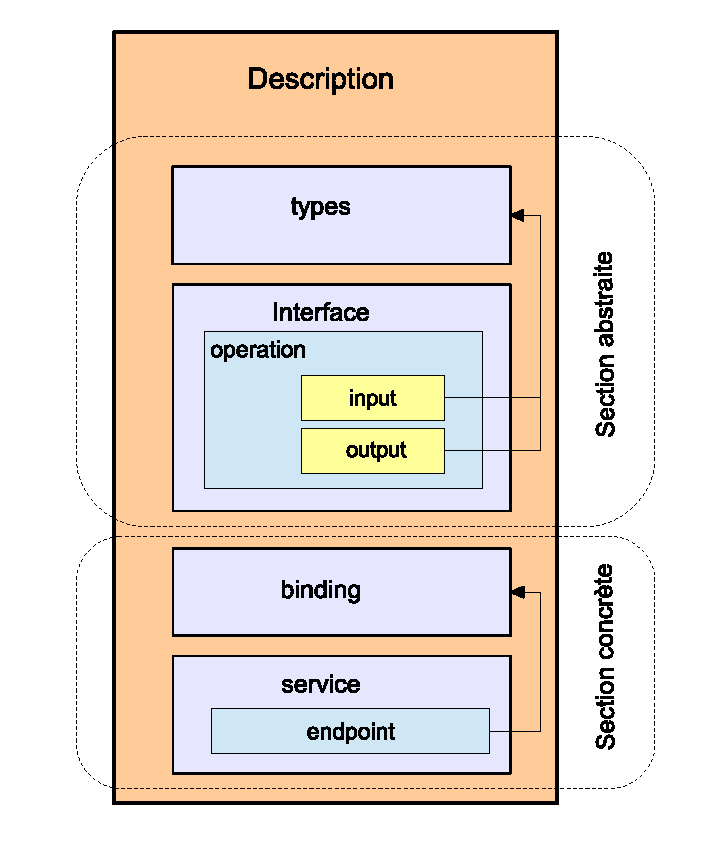
\includegraphics[width=0.6\textwidth]{figs/wsdl-document-structure.eps}
    \caption{Structure d'un message \textsc{WSDL}}
    \label{fig:wsdl-document-structure}
\end{figure}

%%% Local Variables:
%%% mode: latex
%%% TeX-master: "../main"
%%% End:


  Le langage de description de services Web \acrshort{wsdl}
  \cite{chinnici2007web} fournit un modèle ainsi qu'un langage basé
  sur \textsc{XML} de description de services Web. Un fichier
  \textsc{WSDL} comprend une description des fonctionnalités d'un
  service, mais il ne se préoccupe pas de l'implantation de celles-ci.
  Il contient aussi des informations concernant la localisation du
  service, ainsi que les données et les protocoles à utiliser pour
  l'invoquer. En pratique, le document \textsc{WSDL}
  \footnote{\url{http://www.w3.org/TR/wsdl20/}} est un document
  \textsc{XML} qui se divise en deux parties \cite{elie2010} :

  \SpecialItem
  \begin{itemize}
  \item La définition \textbf{abstraite} de l'interface du service
    avec les opérations supportées par le service Web, ainsi que leurs
    paramètres et les types des données.

  \item La définition \textbf{concrète} de l'accès au service avec la
    localisation, par une adresse réseau du fournisseur de service
    \footnote{Service Endpoint}, et les protocoles spécifiques
    d'accès.
  \end{itemize}

  La partie abstraite d'un document \textsc{WSDL} contient deux
  sous-parties:

  \SpecialItem
  \renewcommand{\descriptionlabel}[1]{\hspace{1.5cm}\texttt{#1}}
  \begin{description}
  \item[<Types>]: décrit sous la forme d'un schéma \textsc{XML} les
    types des données échangées entre le client et le fournisseur de
    services \cite{part20012}.

  \item[<Interface>]: Les interfaces\textsc{WDSL} offrent une manière
    abstraite de décrire la fonctionnalité du service, ils ont défini
    les opérations (éléments \texttt{<operation>}) en terme de
    paramètres d'entrée et de sortie sous frorme d'un un modèle
    d'échange de message \textit{(message exchange
      pattern)}. \textsc{WSDL} contient huit modèles de messages
    prédéfinis, mais on peut facilement définir de nouveaux.
  \end{description}

  La définition concrète d'un document \textsc{WSDL} est constituée
  de:

  \SpecialItem
  \renewcommand{\descriptionlabel}[1]{\hspace{1.5cm}\texttt{#1}}
  \begin{description}
  \item[<Binding>]: L'élément \texttt{Binding} reprend les opérations
    de l'élément \texttt{<Interface>} et leurs associe un protocole de
    transfert et des spécifications des formats de données de message.

  \item[<Service>]: Cet élément définit la localisation du service Web
    décrit. Pour chaque interface décrite, un élément service lui est
    associé. Le sous-élément \texttt{<endpoint>} définit un port
    d’accès en référençant l'élément \texttt{<binding>} associé et en
    déclarant l'\textsc{URL} localisant le service (avec l'attribut
    \texttt{<address>}).
  \end{description}
  % parler sur la limitation de la description syntaxique de WSDL,
  % réferencer les \ref{sec:ws-description}
  \newpage
  \subsection{Découverte: UDDI}
  \label{sec:uddi}
  % TODO
  \acrshort{uddi} \cite{clement2004uddi} est une standardisation pour
  la publication et la découverte de services Web initialement conçue
  et spécifiée par le Consortium de standards
  OASIS\footnote{\url{https://www.oasis-open.org}}, il est le résultat
  d'un accord d'un ensemble d'industriels
  Ariba\footnote{\url{http://www.ariba.com/}}, IBM, Microsoft, etc en
  vue de devenir le registre standard de la technologie de services
  Web.

  \textsc{UDDI} complète les technologies basiques de services Web en
  permettant de créer un \textbf{annuaire} permettant de localiser sur
  le réseau le services web recherchés, les services référencés dans
  \textsc{UDDI} sont accessibles par l'intermédiaire du protocole de
  communication \textsc{SOAP}, et la publication des informations
  concernant les fournisseurs et les services doit être spécifiée en
  \textsc{XML} afin que la recherche et l'utilisation soient faites de
  manière \textbf{dynamique} et \textbf{automatique}.

  Un \textsc{UDDI} peut appartenir à un domaine public comme internet
  ou tout autre réseau accessible à un nombre non limité
  d'utilisateurs, comme il peut appartenir à un domaine restreint
  comme l'intranet d'une entreprise ou d'un groupe d'entreprise.

  % TODO ajouter la description dans  denayer2004decouverte

  Les données stockés dans l'\textsc{UDDI} sont structurées (en
  \textsc{XML}) et organisées en trois parties connues:

  \SpecialItem
  \begin{description}
    \item[Pages blanches]: fournissent des descriptions générales sur
      les fournisseurs de services à savoir le nom de l'entreprise qui
      fournit le service, son identificateur commercial, ses adresses,
      etc.

    \item[Pages jaunes]: comportent des descriptions détaillées sur
      les fournisseurs de services catalogués dans les pages blanches
      d'une de façon taxonomique (selon secteurs d'activités par
      exemple).

    \item[Pages vertes]: fournissent des informations techniques sur
      les services Web catalogués. Ces informations incluent la
      description du service, les adresses \textsc{URL}, du processus
      de son utilisation et des protocoles utilisés pour son
      invocation.
  \end{description}

  % TODO: talk about OWL-S and why UDDI approach is semantically poor
  % TODO : Conclure cette subsection par la mention du problème de la
  % découverte automatique de services Web et l'insuffisance de la
  % description syntaxique.
  % \newpage

  % critiquer la découvert manual de services dans UDDI
  % référencer \ref{sec:ws-localisation}

\section{Description de services web}
\label{sec:ws-description}

% Un service Web consiste à la définition d'une entité logiciel
% modulaire, \textit{auto-descriptive} et \textit{autonome}
% \textit{accessible} via Internet \cite{curbera2001web}. Dans la
% section précédente, nous avons vu l'architecture de base de services
% Web et la pile protocolaire pour la mise en place d'une telle
% architecture.

Une description du service Web est un document par lequel le
fournisseur de services communique au client les spécifications pour
invoquer le service Web \cite{lopez2008selection}. Malgré les
améliorations apportées au standard \textsc{WSDL} dans son deuxième
version \cite{chinnici2007web}, la description du service reste
uniquement au niveau fonctionnel, c'est-à-dire qu'elle contient la
manière dont on peut utiliser le service et non ce que fait le
service, le standard \textsc{WSDL} est limité à l'énumération des
opérations et à la description des types des paramètres d'entrée et de
sortie associés, elle ne caractérise pas la sémantique de la
fonctionnalité accomplie par le service.

Par conséquent, la description \textsc{WSDL} reste insuffisante lors
des processus de sélection, découvert et de la composition. Pour
pallier cette Difficulté, plusieurs approches
\cite{sivashanmugam2003adding,mcilraith2001semantic,
  mcilraith2003bringing, fensel2002web} proposent de rajouter une
couche sémantique au dessus de \textsc{WSDL} complétant la description
syntaxique par des précisions sémantiques.

%!TEX root = ../main.tex
\begin{figure}[h]
    \centering
    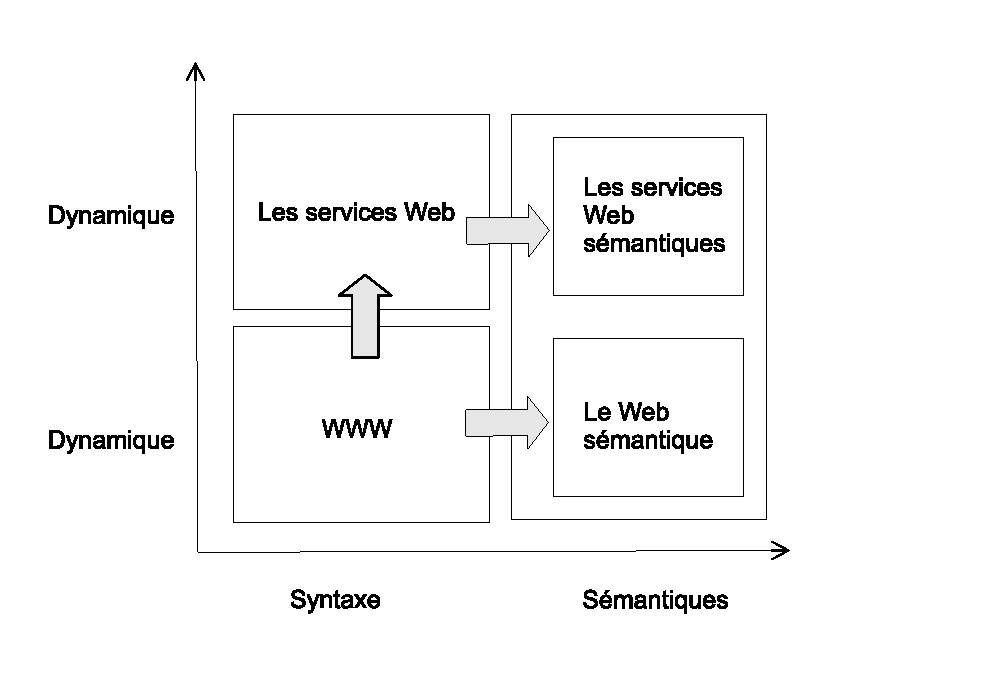
\includegraphics[width=1\textwidth]{figs/3w_to_sws.eps}
    %TODO translate
    \caption{Web evolution to Semantic Web services \cite{fensel2002semantic}.}
    \label{fig:3w_to_sws}
\end{figure}
\newpage
Les services Web enrichis par des métadonnées supplémentaires
exprimant leur la sémantique sont appelés \textit{les services Web
sémantiques} \cite{fensel2002semantic, mcilraith2001semantic}. Les
services de Web sémantique sont le résultat de l'évolution Web dans
deux directions \cite{bartalos2011effective} (illustré dans La
figure\ref{fig:3w_to_sws}):

\begin{enumerate}
  \item L'interopérabilité dynamique des éléments sur le Web.
  \item L'amélioration de la description syntaxique services Web
\end{enumerate}

Dans cette section nous allons présenter les diverses approches
sémantiques visant à préciser la description d'un service en insistant
sur les approches d'annotation sémantique et sur les ontologies de
services.

La notion du Web sémantique est abordée brièvement dans l'annexe
\ref{annexe:semantic-web}.

  \subsection{Annotations sémantiques}
  \label{sec:semantic-annot}

  L'annotation sémantique consiste à enrichir et à compléter la
  description d'un service. Elle établit des correspondances entre des
  éléments de la description et des concepts d'un ensemble
  d'ontologies de références. Une ontologie de référence permet de
  représenter un domaine par des structures interprétables par une
  machine. Deux modèles principaux suivent l'approche d'annotation
  sémantique, à savoir \textsc{WSDL-S} et \textsc{SAWSDL}
  \cite{elie2010}.

    \subsubsection{WSDL-S}
    \textsc{WSDL-S} \cite{akkiraju2005web} est le résultat d'un
    travail collaboratif entre IBM, laboratoire LSDSI et l'iniversité
    de Geogia \footnote{\url{http://www.uga.edu/}}.  La spécification
    a devenue une recommandation \textsc{W3C} depuis 2005. Son
    objectif principal est de fournir un processus d'annotation
    sémantique compatible avec les technologies
    existantes. Pratiquement, Le méta-modèle \textsc{WSDL-S} repose
    sur les capabilités du modèle \textsc{WSDL} en rajoutant trois
    éléments majeurs \texttt{<category>}, \texttt{<effect>} et deux
    attributs \texttt{modelReference} et \texttt{schemaMapping}. Les
    éléments introduits permettent de rajouter des informations qui
    n'étaient pas prises en compte dans \textsc{WSDL} comme \emph{les
      préconditions} et \emph{les effets} d'une opération. Tandis que
    les attributs permettent de référencer des concepts dans des
    ontologies de référence, ces préconditions et effets ensemble avec
    les annotations sémantiques des éléments \texttt{<inputs>} et
    \texttt{<outputs>} permet de l'automatisation du processus de
    découvert de services.

    \subsubsection{SAWSDL}
    La spécification \acrshort{sawsdl} \cite{kopecky2007sawsdl} est la
    suite de \textsc{WSDL-S} et il partage les mêmes principes de ce
    dernier. issue d'initiative du groupe de travail d'annotations
    sémantiques pour \textsc{WSDL}
    \footnote{\url{http://www.w3.org/TR/sawsdl/}} et soumise au
    \textsc{W3C} en 2007, \textsc{SAWSDL} définit un mécanisme
    d'annoter sémantiquement les interfaces et les opérations
    \textsc{WSDL}, ainsi que les types \textsc{XML schema} en les
    reliant à des concepts dans une ontologie. Cette annotation repose
    sur la définition d'attributs étendant le standard de
    description. Les annotations sémantiques référencent des
    ontologies pré-existantes. Le mécanisme d'annotation de
    \textsc{SAWSDL} est indépendant de tout langage de représentation
    \cite{lopez2008selection} d'ontologies.

    \textsc{SAWSDL} propose deux sortes d'annotations sémantiques: une
    pour identifier le concept sémantique (représentée par l'attribut
    \texttt{modelReference}) et une autre pour faire le lien entre le
    concept et le document \textsc{WSDL} (représentée par les
    attributs \texttt{liftingSchemaMapping} et
    \texttt{loweringSchemaMapping}).

  \subsection{Ontologies de services}
  \label{sec:ont-services}

  Une ontologie de services saisit les différents aspects liés à la
  description de services et leur utilisation à travers un ensemble
  de concepts, de propriétés et de relations entre eux. Deux modèles
  d'ontologies de services sont décrits dans cette sous-section
  \textsc{OWL-S} et \textsc{WSMO} \cite{elie2010}.

    \subsubsection{WSMO}
    \label{sec:wsmo}

    \acrshort{wsmo} \cite{de2005web} est une modèle conceptuel basé
    sur la spécification \acrshort{wsmf} \cite{fensel2002web} (voir
    \ref{sec:wsmf}) pour la description des divers aspects liés aux
    services Web sémantique. Le but de \textsc{WSMO} est d'automatiser
    le cycle de vie de services web (publication, sélection,
    découverte, composition, etc.) afin de résoudre le problème de
    l'intégration de services Web en définissant une technologie
    cohérente pour description de services Web sémantique.

    Pour formaliser \textsc{WSMO}, le groupe de travail mis au point
    le langage de modélisation \acrshort{wsml} \cite{de2006web} et a
    défini plusieurs variantes de celui-ci, chacun basé sur différents
    formalismes.

    \textsc{WSMO} est constitué de quatre composants: les services
    web, les buts, les ontologies et les médiateurs. Ce modèle permet
    de réaliser un couplage faible entre les services web en utilisant
    un ensemble de médiateurs. Ces derniers assurent les tâches
    d‘intégration d'ontologies, de découverte de services, de
    composition, etc.

    \subsubsection{OWL-S}
    \label{sec:owl-s-1}

  % TODO: elaborate
  \subsection{L'aspect fonctionnel et non fonctionel de description}
  \label{sec:func-vs-non-func}
  % TODO  move this section the first section of the chapter-3
  {\color{red}
    \cite{el2014cbr4wsd}
  }

  Il existe deux aspects de description de services Web:

    \subsubsection{L'aspect fonctionnel}
    \label{sec:aspect-fonctionnel}

    \subsubsection{L'aspect non fonctionnel}
    \label{sec:aspect-non-fonctionel}

\newpage
\section{Découverte de services web}
\label{sec:ws-discovery}
La découverte de services Web présente un axe de recherche
important. Divers mécanismes de découverte ont été proposés dans la
littérature et plusieurs définitions sont attribuées à ce
concept. Booth \textit{el al.}  décrivent le processus de découverte
comme étant l'acte de \textit{``localisation d'une description
  compréhensible par la machine d'un service éventuellement inconnu au
  préalable écrivant certains critères fonctionnels ''}
\cite{booth2004web}.

\begin{figure}[h]
    \centering
    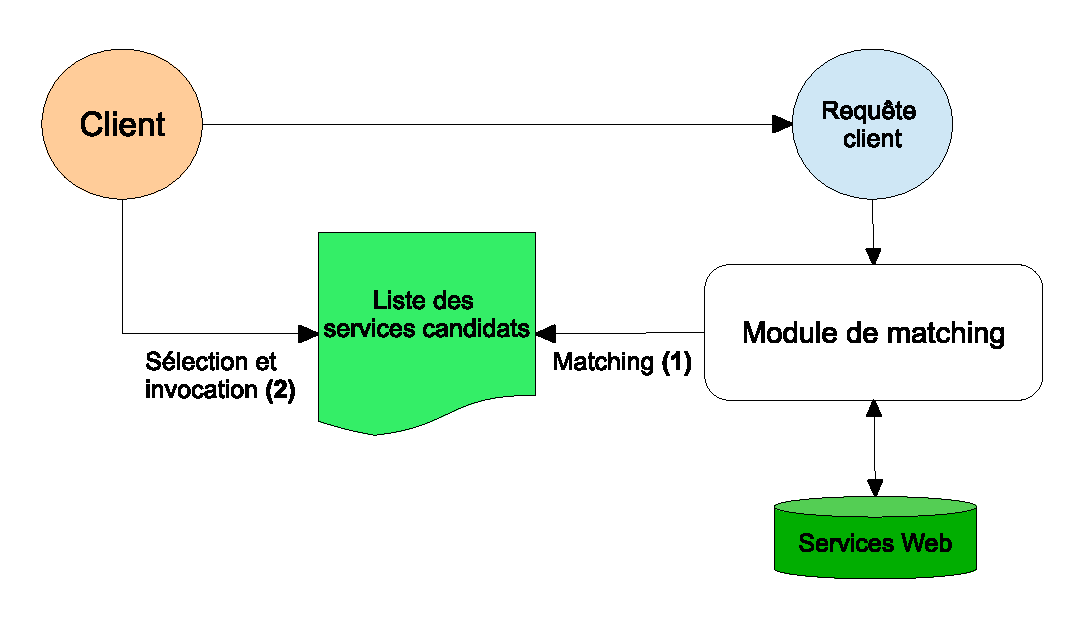
\includegraphics[width=0.55\textwidth]{figs/ws-discovery-with-matching.eps}
    \caption{Découverte des services Web}
    \label{fig:ws-discovery-with-matching}
\end{figure}

%%% Local Variables: 
%%% mode: latex
%%% TeX-master: "../main"
%%% End: 


Un processus de découverte de service web s'effectue en deux phases
principales (illustrés dans la figure
\ref{fig:ws-discovery-with-matching}). Premièrement, un module de mis
en correspondance (\textit{Matching}) renvoie tous les services Web
candidats selon le degré de similitude entre les services disponibles
et les exigences spécifiés par la requête (aspect fonctionnel). La
deuxième étape consiste à sélectionner et invoquer le service le plus
satisfaisant (aspect non fonctionnel). Plusieurs critères peuvent être
utilisés pour catégoriser les approches de découverte \cite{elie2010}:

\begin{enumerate}
\item la localisation de services (centralisation/décentralisation
  des annuaires).
\item Le degré d'automatisation du processus de la découverte.
\item le principe de l'algorithme de \textit{Matching}.
\end{enumerate}

Dans cette section nous présentons les différentes approches de
localisation de services basées sur des modèles centralisés ou des
modèles distribués. Ensuite nous classifions les approches de
découverte selon le degré d'automatisation du traitement des
données. Le dernier critère de classification sera présenté dans la
prochaine section \ref{sec:ws-matching}.

\subsection{Localisation de services}
\label{sec:ws-localisation}
  La découverte consiste principalement à localiser les descriptions
  de services répondant à une requête client. Les approches de
  localisation de services récurrentes dans la littérature sont
  classées en deux catégories, à savoir les approches centralisées et
  les approches décentralisées ou distribuées
  \cite{garofalakis2004web}.

  \renewcommand{\descriptionlabel}[1]{\hspace{0.1cm}\textbullet~\textsf{#1}}
  \begin{description}
  \item [Approches centralisées:] Les premières versions
    d'\textsc{UDDI} \cite{clement2004uddi} (présenté dans
    \ref{sec:uddi}) reposent sur une approche \textit{centralisée} de
    publication et découverte de services Web. le registre
    \textsc{UDDI} définit un modèle de représentation des données et
    des méta-données nécessaires à la publication, reposent sur
    \textit{un seul annuaire} qui peut être géré par un module de mise
    en correspondances \textit{(matchmaker)}.

  \item [Approcehs décentralisées:] Les approches décentralisées de
    découverte de services \cite{rompothong2003query,
      sivashanmugam2004discovery, paolucci2003using, schmidt2004peer,
      verma2005meteor, sahin2005spider} consistent à mettre en place
    une \textit{fédération} d'annuaires \textsc{UDDI} agissant comme
    une couche d'abstraction reliant plusieurs instances
    d'annuaires. La plupart des approches distribués sont basées sur
    des systèmes pair-à-pair (\textit{peer to peer}) incluant
    \cite{schmidt2004peer, verma2005meteor, sahin2005spider}.

    La dernière version d'\textsc{UDDI} \cite{oasis2005specification}
    (\textit{3.0.2}) reprend le principe d'une fédération d'annuaires
    et décrit un annuaire \textsc{UDDI} comme un ensemble de nœuds
    \textit{(UDDI nodes)} tel que chaque nœud fait partie d'un seul
    annuaire et possède une copie répliquée de schéma globale de la
    fédération. Les nœuds d'un annuaire collaborent pour gérer un
    ensemble de structures de données \textsc{UDDI} et permettre une
    meilleure gestion des requêtes.
  \end{description}

  \subsection{Découverte manuelle/automatique}
  \label{sec:ws-desc:manual-vs-auto}
  Selon le richesse sémantique de la description de services, le
  degré d'intervention de l'utilisateur dans la découverte
  variée. Nous pouvons distinguer les approches manuelles et
  semi-automatique d'une part, et les approches automatiques d'une
  autre part \cite{elie2010,garofalakis2004web}.

  \renewcommand{\descriptionlabel}[1]{\hspace{0.1cm}\textbullet~\textsf{#1}}
  \begin{description}
  \item[Approches manuelles et semi-automatiques:] Dans une découverte
    manuelle, le client utilise un service de découverte pour
    localiser et sélectionner manuellement une description de service
    qui répond aux certains critères fonctionnels. La recherche de
    descriptions dans cette approche est souvent basée sur une simple
    comparaison syntaxique entre les mots clés de la requête et les
    descriptions de services disponibles, ce qui nécessite
    l'intervention de l'utilisateur pour vérifier la pertinence et la
    fiabilité des résultats de la recherche et sélectionner le service
    Web qui répond au mieux à ses exigences.

    % Verma \textit{et al.}  \cite{verma2005meteor} dans le cadre du
    % projet \textsc{METEOR-S}, l'infrastructure présente un degré
    % d'automatisation plus avancé qu'une simple recherche dans un
    % annuaire \textsc{UDDI}. En effet, l'enrichissement sémantique des
    % fichiers de description de services Web permet une découverte
    % semi-automatique et plus précise
    .

  \item[Approches automatiques:] La découverte automatique de services
    qui répond à un besoin donné est considéré comme une étape
    cruciale vers l'intégration dynamique et évolutive de services
    Web. On entend par découverte automatique la possibilité de
    localiser automatiquement un Web service qui répond à des besoins
    particuliers, Différentes approches ont été proposées dans la
    littérature pour réaliser la découverte dynamique de services
    \cite{paolucci2002semantic, bernstein2002discovering,
      mandell2003bottom,
      benatallah2005automating,keller2005automatic}. Dans
    \cite{mandell2003bottom} les auteurs présentent une approche
    d'automatisation de la découverte de services modélisés en
    \acrshort{bpel} (voir \ref{sec:bpel}) dans le but d'une
    composition plus dynamique. Les auteurs proposent d'étendre la
    description \textsc{BPEL} par l'intégration d'une description
    sémantique \textsc{OWL-S} (voir \ref{sec:owl-s}) de type
    \textit{service profile} et la mise en place d'un module de
    \textit{Matching} sémantique équipé par un raisonneur
    automatique. Autrement, Keller \textit{et al}
    \cite{keller2005automatic} étudient un modèle de localisation
    automatique de services Web décrits via le modèle \textsc{WSMO}.
  \end{description}

\section{Matching de services Web}
\label{sec:ws-matching}
Le \textit{Matching} (ou le \textit{Matchmaking}) de services Web est
définie comme un processus qui nécessite un annuaire de services de
prendre une requête en entrée, et de revenir tous les services qui
peuvent satisfaire les exigences spécifiées dans la requête d'entrée
\cite{li2004software}. Cette opération nécessite la recherche de
similarités indiquant le degré de rapprochement entre les paramètres
descriptives fonctionnels et non fonctionnels
(~\ref{sec:func-vs-non-func}) de services référencés d'une côté, et
les paramètres de la requête client d'une autre.

Le calcul de similarité peut être basé sur des données syntaxiques ou
sémantiques plus expressives \cite{elie2010}. Dans la suite nous
résumons les approches de \textit{Matching} de services Web
rencontrées dans la littérature.

  \subsection{Matching syntaxique}
  \label{sec:matching-syntactique}
  Les approches de \textit{Matching} synatxique sont basées sur la
  description \textbf{syntaxique} de services (\textsc{WSDL})
  référencés dans un annuaire \textsc{UDDI} \cite{clement2004uddi}. Le
  client envoie une requête constituée de mots clés, cette requête est
  ensuite comparée avec les mots clés du registre \textsc{UDDI}. Un
  ensemble de descriptions de services Web sous forme des documents
  \textsc{WSDL} (ou un ensemble des \textsc{URL} de ces derniers) est
  ensuite donné comme résultat de recherche, le client sélectionne le
  service Web qui répond au mieux à ses exigences.

  Liang \textit{et al.} \cite{DBLP:journals/jwsr/LiangCSCL04}
  emploient la base de données lexicale \textit{WordNet}
  \footnote{\url{http://wordnet.princeton.edu/}}
  \cite{miller1990introduction} pour enrichir les mots clés de la
  requête avec des synonymes. Ceci permet d'améliorer la qualité des
  résultats.

  Sajjanhar \textit{et al.} \cite{sajjanhar2004algorithm} utilisent
  des méthodes d'algèbre linéaire pour rendre le \textit{Matching} par
  mots clés plus efficace. leur approche consiste à construire une
  matrice contenant des informations sur tous les services Web qui ont
  des mots communs dans leur description. Ensuite, une décomposition
  en valeurs singulières est appliquée à cette matrice pour obtenir
  toute description de service Web qui a une relation avec la requête
  de recherche.

  Malgré sa simplicité et sa facilité d'implémentation, les approches
  syntaxiques présentent plusieurs limitations:

  % TODO: enhance
  \begin{itemize}
  \item un faible taux de rappel et de précision à cause de
    l'ambigüité du langage naturel.
  \item La nécessité de l'intervention de l'utilisateur.
  \end{itemize}
  % TODO: introduire le matching sémantique.

  \subsection{Matching sémantique}
  \label{sec:matching-semanique}
  De récents travaux se sont focalisés sur la description sémantique
  de services Web dans le but d'adresser les insuffisances des
  approches purement syntaxiques (voir \ref{sec:ws-description}). Les
  ontologies sont les modèles les plus utilisés pour la représentation
  sémantique de services Web. Dans ce type de découverte, le
  prestataire de service doit fournir des annotations sémantiques pour
  ses services publiés. La description sémantique se rapporte à la
  définition abstraite de services comprenant les types
  d'\textit{entrées/sorties}.

  Un \textit{Matching} sémantique consiste à identifier un certain
  degré de similitude entre les différents concepts sémantiques qui
  décrivent le service requis (la requête) et celles de services
  publiés.

  Les approches de calcul de similarités sémantique reposent sur des
  modèles de description sémantique. Par la suite nous résumons deux
  approches majeures, basées respectivement sur le modèle
  \textsc{WSMO} et sur le modèle \textsc{OWL-S}.

    \subsubsection{Matching sémantique basé sur WSMO}
    \label{sec:match-wsmo}
    \cite{paolucci2002semantic, keller2004wsmo}

    \subsubsection{Matching sémantique basé sur OWL-S}
    \label{sec:match-owls}
    \cite{paolucci2002semantic,benatallah2003request,
        benatallah2005automating, martin2004owl}

\newpage
\section{Conclusion}
% faire un petit récapitulatif sur les technologies de services web
% rappeler de notre problème principale : composition de services web

%%% Local Variables:
%%% mode: latex
%%% TeX-master: "../main"
%%% End:
